\documentclass[12pt, letterpaper]{article}
\usepackage[utf8]{inputenc}
\usepackage{amsmath} 
\usepackage[margin=1in]{geometry}
\usepackage{mathtools}
\usepackage{listings}
\usepackage{wrapfig}
\DeclarePairedDelimiter\ceil{\lceil}{\rceil}
\DeclarePairedDelimiter\floor{\lfloor}{\rfloor}

\title{Application of Genetic Algorithms in Optimizing Traffic Flow}
\author{Matthew Bianchi and Drew Neely}
 
\begin{document}

\maketitle

Our group chose to investigate the problem of traffic. 
The average urban driver will spend a lot of time stuck in traffic, so reducing this wasted time can improve productivity of society, allow people to have more time to themselves not lost sitting in gridlock, and reduce frustration on the road.
The goal of this project was to choose a traffic light pattern for a specific city sector that minimizes the amount of time cars spend stopped, what we will hereon refer to as wait time.
We attempted to optimize traffic lights at a set of several intersections within a few city blocks, reducing the wait time of all cars and increasing intersection flow in that section of the city. 
In order to solve this, we used reinforcement learning techniques, rewarding minimizing wait time and increasing flow through the intersection. 
We used simulated datasets and trained on a variety of scenarios, such as traffic patterns with rush hour, non-uniform traffic, and on city grids of varying sizes. 
We chose to use an evolutionary algorithm, as the nature of the problem suggests using a hill climbing algorithm where repeated small improvements build up gradually over time. 

There are many factors to consider when trying to optimize the flow of traffic, many of which involve the layout, size, and laws of the roads.
We chose to hold most of these variables constant for the sake of simplicity by only considering scenarios with two-way roads with one lane in each direction laid out in a grid pattern. 
We assume all roads have the same speed limit, all cars drive at exactly the speed limit, time that cars spend accelerating from a stop or decelerating to a stop have no affect on traffic flow, and the drivers make no mistakes (eg. not noticing when the light turns from red to green).

\section*{Method}

We chose to approach this problem as a reinforcement learning problem.
Our goal was to train using a genetic algorithm with the intent to minimize a heuristic value, namely the total waiting time of all cars at intersections.
The genetic algorithm we created initializes with a randomly seeded set of traffic patters as the first generation.
The quality of each traffic pattern is evaluated by running a simulation, and some number of the patterns are picked (with repitition) to become a part of the next generation such that the probability of each pattern being picked is proportional to its quality.
At each iteration, the selected traffic patterns are ``mutated'' so that a few of the traffic signals are randomly changed.
Genetic algorithms are specifically well-suited for optimization problems, as the best of these samples will ``survive'' to make it into future generations and the algorithm will slowly improve due to random variation.
Since we always keep the best result of our samples, we will never become less optimal in our new generation of samples, and because of our mutations, we have a chance in every generation of randomly becoming better.
Over time, this will approach an optimal value.

Many genetic algorithms used crossover between generations in which two randomly selected solutions are made into one by taking elements from each and combining them.
We chose not to implement crossover in our algorithm.
We felt that the algorithm with only mutation was sufficient for this problem and gave satisfactory results.


\section*{Data}

\begin{wrapfigure}{r}{0.45\textwidth}
\begin{center}
	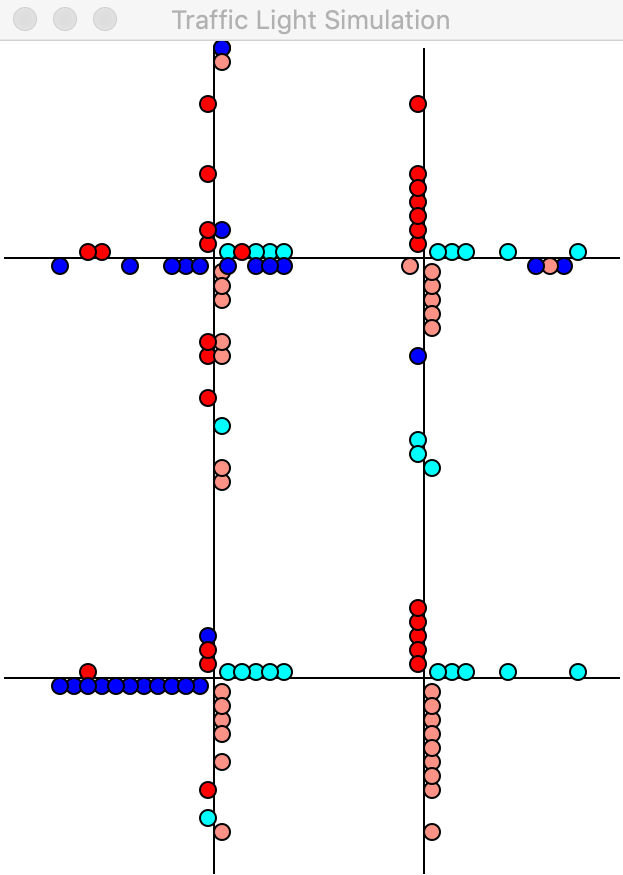
\includegraphics[scale=0.5]{screenshot.png}
	\caption{A sample simulation graphic}
\end{center}
\end{wrapfigure}

For this project, we created a simulator for the data.
This simulator consisted of multiple intersecting roads, with cars traversing along them.
Cars move along the road until there is a car stopped in front of them or until they reach an intersection in a state which does not allow them to pass.
In these cases they must wait for the path in front of them to clear.
Each road had a spawner at its start, which controls the rate of cars entering the simulation.
Each intersection also had designated behaviors for cars, such as ``Most cars traveling North will go straight'' or ``Cars will only turn right at this intersection.''
The genetic algorithm had the responsibility of learning the patterns these cars will take and adjusting the light pattern to match.

We defined intersection states as the paths through the intersection which had a green light, allowing cars attempting to travel in that direction to proceed through the intersection.
Each car entering the intersection has the option of going straight, turning left or turning right, the probabilities of which were set in the simulation files.
In a given state, each exiting road for the intersection was used exactly once, and none of the paths in the intersection were allowed to cross each other (for example, a left turn across oncoming straight traffic).
Our simulator had a total of 17 different possible states for an intersection.
Some examples include one road having full right of way and the road to its left turning right and roads travelling in the opposite directions going straight and turning right.
The pattern of these intersection states was what our genetic algorithm evaluated and mutated.

We measured success as improvement over true random intersection behavior.
On the larger maps, we sought at least a 20\% improvement on average over this random behavior.
We quantified improvement as a reduction in waiting time, which was the parameter we trained on.
We also had one case where our goal was to remove wait time completely, that being a case where all cars turn right at an intersection.
This case matches one of the states an intersection could be in, so we tested to see if the algorithm would find this case.


\section*{Experimental Results}

We tested the ability of the Genetic Algorithm to reduce waiting times in the simulation on three different scenarios. 
The first scenario (shown in Figure 1) consisted of two vertical road and two lateral roads. 
Upon approaching every intersection a car had a 70\% chance of going straight, and a 15\% chance of turning in either direction. 
The traffic light pattern generated by 100 generations of the genetic algorithm reduced the waiting time by more than 25\% from the average waiting time of a randomly generated traffic light pattern. 

The second scenario consisted of three vertical roads and three lateral roads. 
The way the cars entered the map and the choices the cars made at each intersection were set so that a particular path through the map had much more traffic than other roads. 
This is representative of a traffic pattern that may be expected in a real-world scenario. 
The genetic algorithm yielded more than 16\% improvement from the average randomly generated traffic pattern. 

The third scenario we chose to test the algorithm on was chosen specifically because it has an optimal traffic pattern in which no car must wait at any time. 
This scenario consisted of one intersection where every approaching car will turn right.
Since the state of the intersection can be set to allow all right turns at one time, the optimal solution is to always be in this state.
The randomly generated traffic pattern caused cars to wait at this intersection for an average of almost two time steps. 
The genetic algorithm found the optimal solution in aproximately 125 generations, allowing all cars to proceed through the intersection with no delay.


\section*{Future Work}
One of the biggest opportunities for improvement comes in improving the simulator.
Our simulator only worked for one-lane, two-directional roads within a city.
However, a simulation which could support multiple lanes, including turn lanes, would allow the algorithm to better optimize the light pattern and improve traffic.
We believe the genetic algorithm would scale to a simulation with multiple lanes very well, allowing for even better improvements.
Another improvement to the simulator would be having cars choose their paths through the city before spawning in, rather than being determined at each intersection individually.
This also serves to improve realism within the simulation and would help our genetic algorithm to create a better light pattern in the city.


\end{document}

